\subsection{a}
The VC-Dim for this interval is equal to: \textbf{}. (explanation to be added)
\subsection{b}
Firstly, it is important to set up our goal. In Vapnik–Chervonenkis dimension, we should search for the largest set shattered by a hypothesis class ($H$). In this case, our $H$ is a circle and everything inside of it is valued 1. Otherwise, it is valued 0. Being so: \\
$$
h_{a,b,r}(x,y)=
        \begin{cases}
			1, & \text{if $(x-a)^2+(y-b)^2 \leq r$}\\
            0, & \text{otherwise}
		 \end{cases}
$$
\bigbreak
Proving the VC-dimension is at least 3:\\
\bigbreak
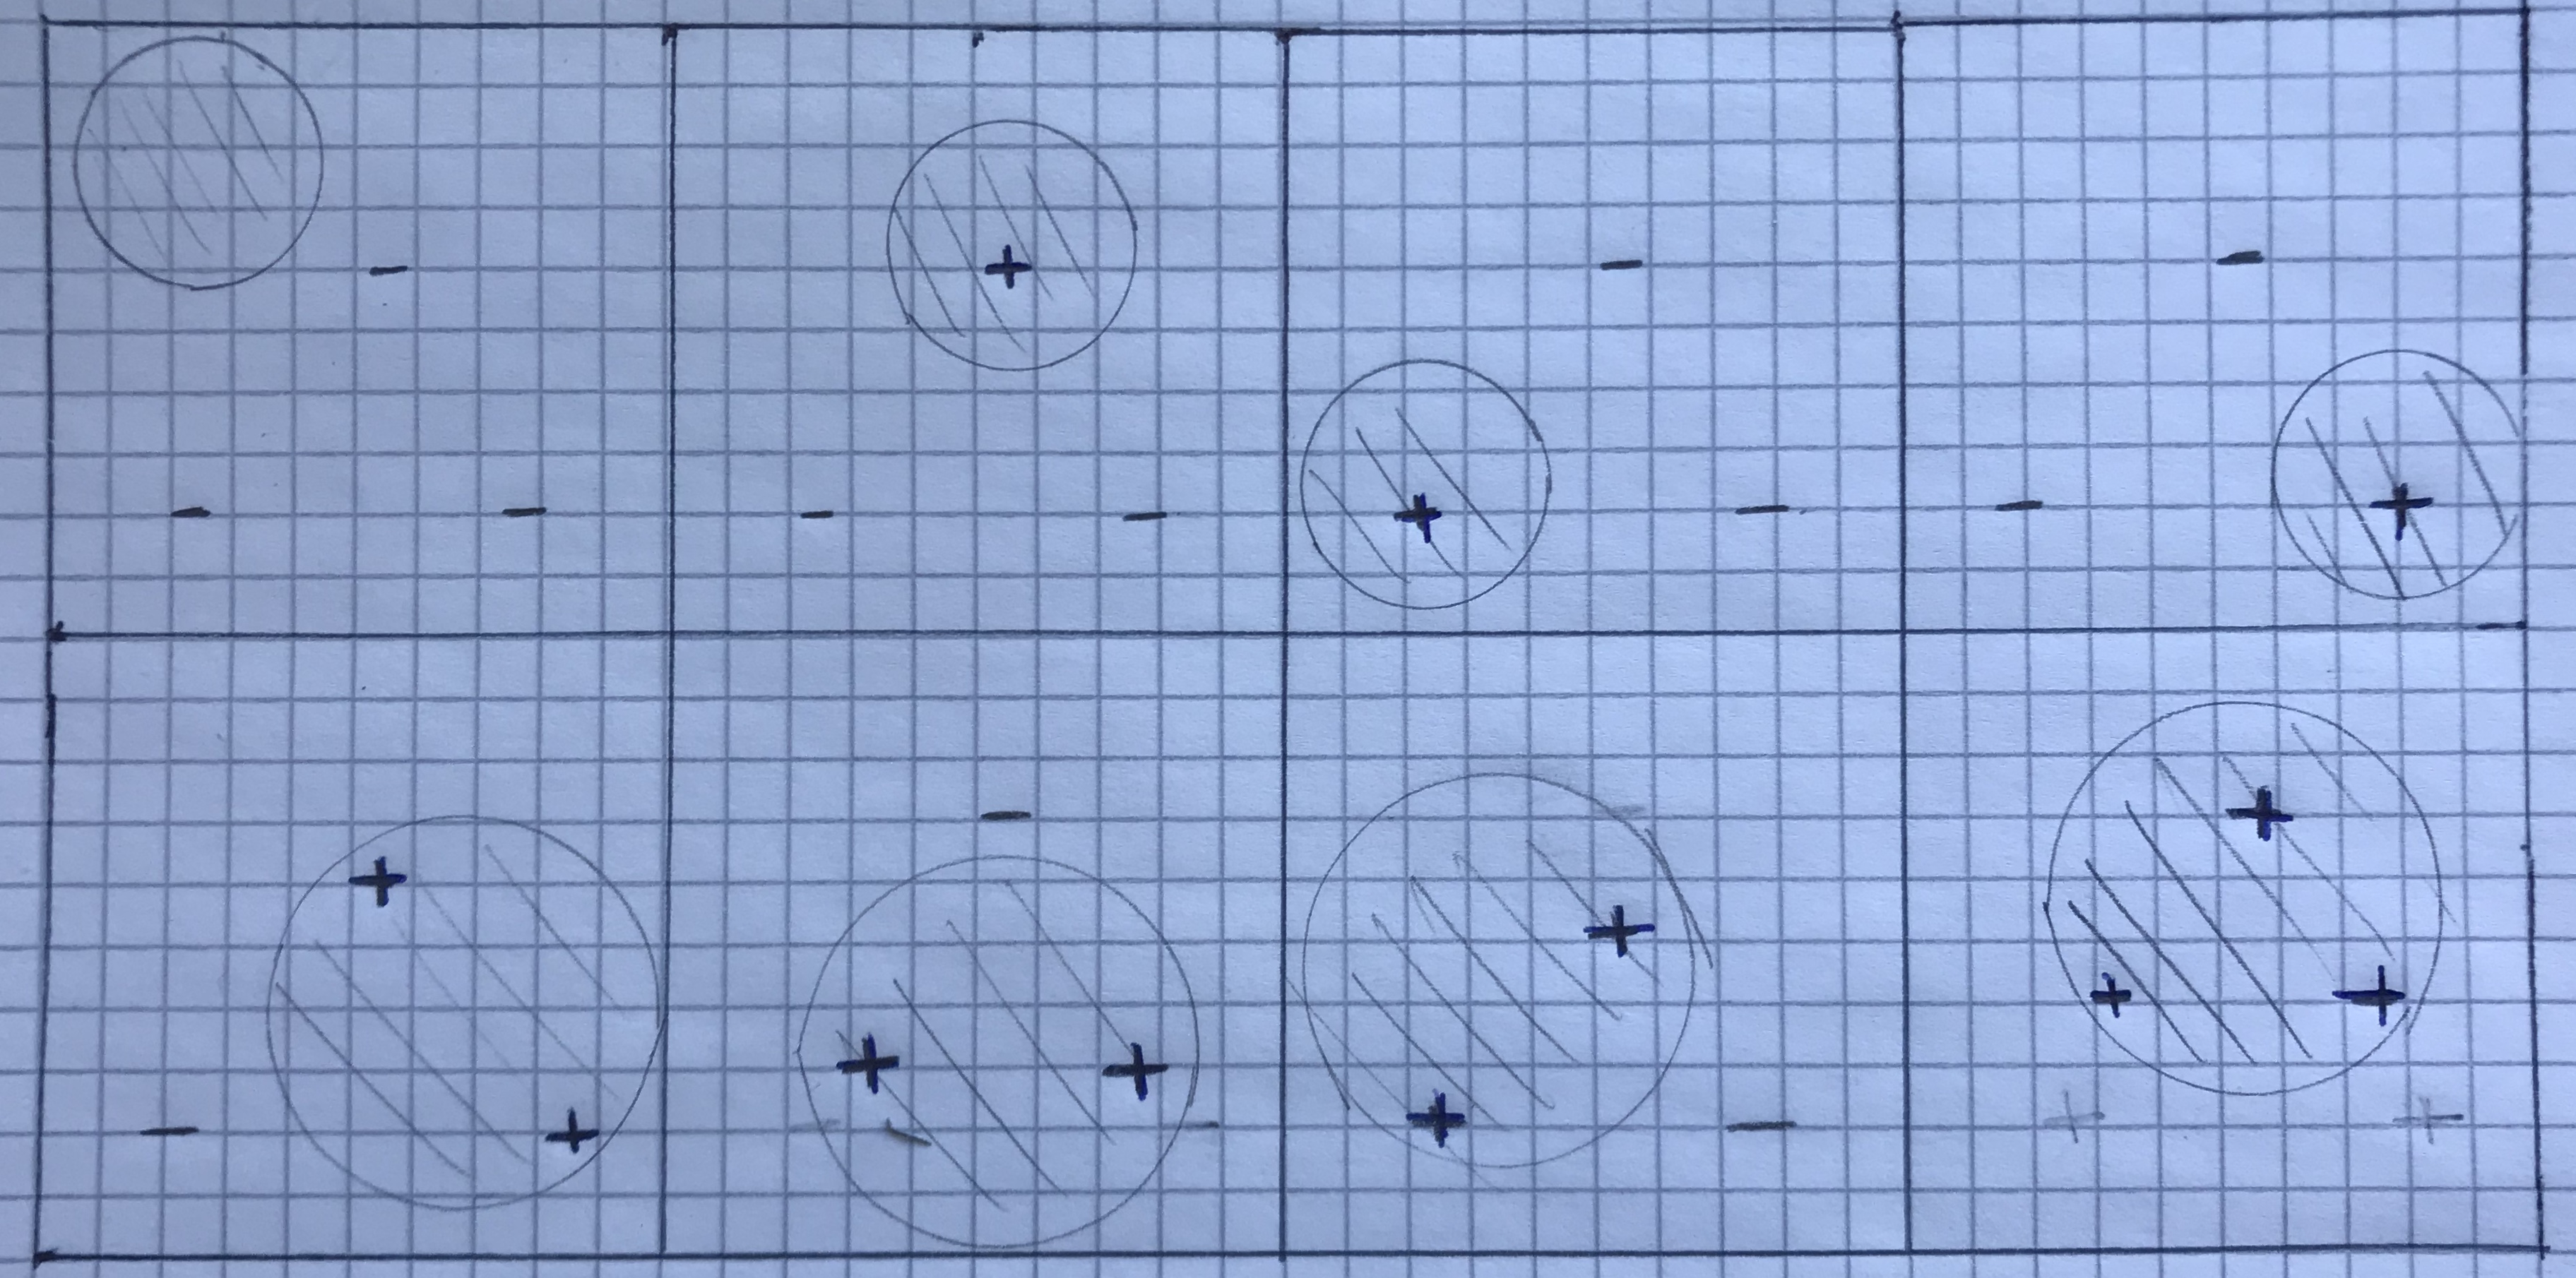
\includegraphics[width=\textwidth,height=\textheight,keepaspectratio]{3dim.jpg}\\
\bigbreak
VC-Dim is at least 3, once we can  draw a circle that have none points, that have any single point, any two points and all of them.\\
\bigbreak
Proving the VC-dimension cannot be 4:\\
\bigbreak
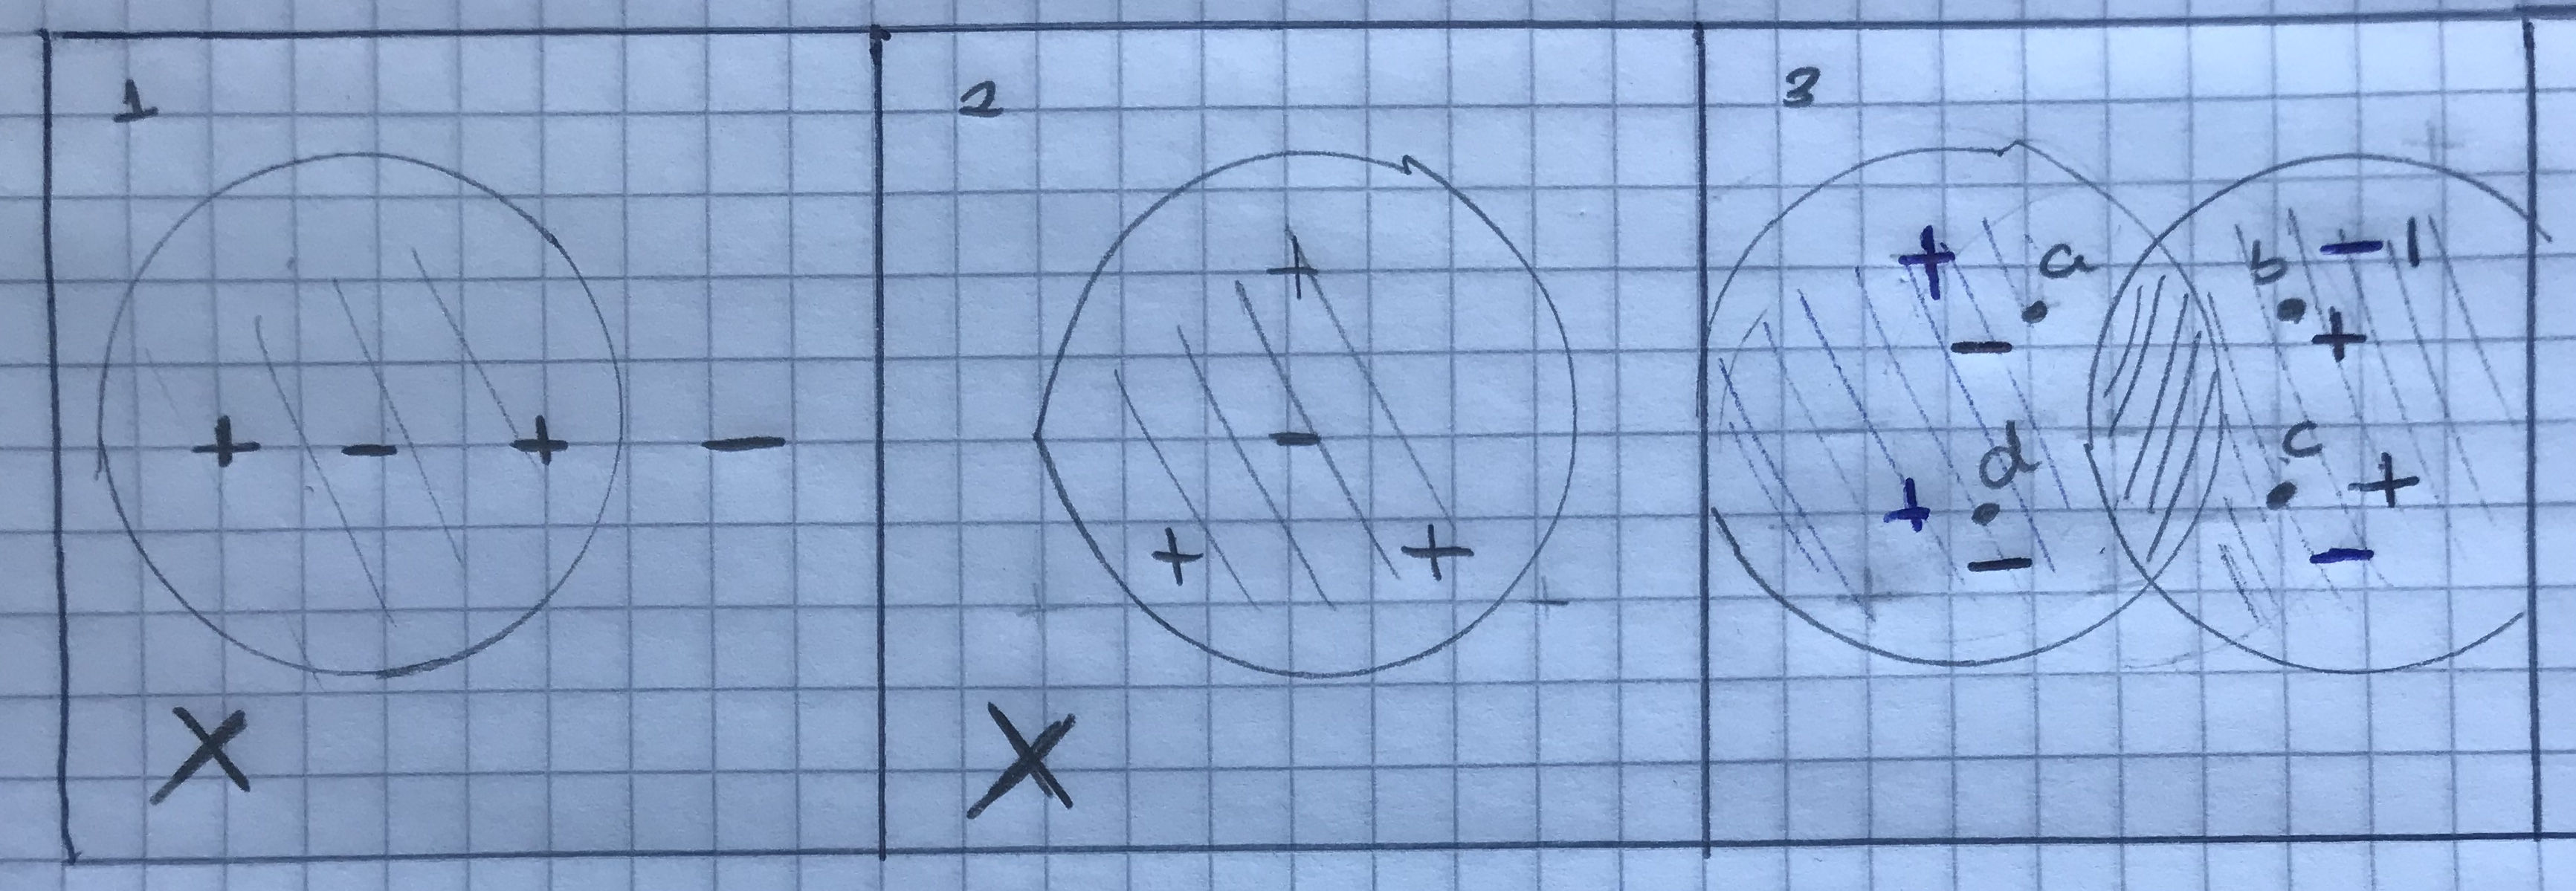
\includegraphics[width=\textwidth,height=\textheight,keepaspectratio]{4dim.jpg}
\bigbreak
VC-Dim cannot be four for the following three reasons:
\begin{enumerate}
  \item Labeling, for instance, $+ - + -$ in this colinear points example is impossible. Several others example with similar arrangement fit in the same explanation. 
  \item Being the convex hull of the four points a triangle, is impossible for the outside points be + and the inside point be -.
  \item Lastly, being the convex hull a quadrilateral defined by points {$a,b,c,d$}, it is not possible to exist a circle that involves $a,c$ and another circle that involves $b,d$. If so, the symmetric difference would consist of 4 disjoint regions, which is indeed impossible for circles.
\end{enumerate}
\bigbreak
Therefore, we can conclude that VC-Dim($H$)$ = 3$. 
